\longsection{%
  \texorpdfstring{%
    Hierarchization on Spatially Adaptive Sparse Grids\\
    with the Unidirectional Principle%
  }{%
    Hierarchization on Spatially Adaptive Sparse Grids
    with the Unidirectional Principle%
  }%
}{%
  Hierarchization on Spatially Adaptive Sparse Grids
  with the Unidirectional Principle%
}{%
  Hierarchization with the Unidirectional Principle%
}
\label{sec:45spatAdaptiveUP}

\minitoc{90mm}{9}

\noindent
In this final section of the chapter,
we further decrease the computational complexity
for the application of the linear operator $\linop$
on spatially adaptive sparse grids
from quadratic to linear time with two algorithms based on the \up.



\subsection{%
  Iteratively Applying the Unidirectional Principle with Iterative Refinement%
}
\label{sec:451iterativeRefinement}

The first algorithm can be applied if two requirements are met:
\begin{itemize}
  \item
  The inverse $\linop^{-1}$ is known and can be efficiently applied.
  
  \item
  There is an operator $\linop'$
  that is ``sufficiently close'' to $\linop$ and can be efficiently applied.
\end{itemize}
For hierarchization with B-splines on sparse grids,
we choose $\linop$ to be the hierarchization
operator given in \cref{eq:hierarchizationSLE} and
$\linop'$ to be the \up directly applied on the
sparse grid.
Both of the assumptions are then satisfied,
as $\linop^{-1}$ is known
(interpolation matrix $\intpmat$ of basis function evaluations)
and $\linop^{-1}$ and $\linop'$ can be applied fast.
The \up $\linop'$ generally produces wrong
results for hierarchical B-splines due to missing coupling points.
However, especially for low B-spline degrees,
$\linop'$ does not deviate too much from the true operator $\linop$.
Below, we will specify a sufficient criterion for the ``closeness.''

\paragraph{Iterative refinement}

Under the two assumptions above, we can apply the procedure given in
\cref{alg:iterativeRefinement}.
The algorithm is equivalent to the well-known method of
\term{iterative refinement,} which has been developed to
stabilize the numerical solution of a linear system
influenced by rounding errors \cite{Higham02Accuracy}.
The operator $\linop'$ acts like a preconditioner,
which is why it is required to be close to $\linop$.
Note that the algorithm is similar to the repeated application
of the method of residual interpolation
(see \cref{sec:433residualInterpolation}) on the whole sparse grid.

\begin{algorithm}
  \begin{algorithmic}[1]
    \Function{$\vlinout = \texttt{iterativeRefinement}$}{%
      $\vlinin$, $\vlinout[(0)]$%
    }
      \State{$\*r^{(0)} \gets \vlinin - \linop^{-1}\vlinout[(0)]$}
      \Comment{initial residual}%
      \For{$m = 0, 1, 2, \dotsc$}
        \State{$\vlinout[(m+1)] \gets \vlinout[(m)] + \linop' \*r^{(m)}$}
        \Comment{update solution}%
        \State{$\*r^{(m+1)} \gets \*r^{(m)} - \linop^{-1} \linop' \*r^{(m)}$}
        \Comment{update residual}%
      \EndFor{}
      \vspace{-1mm}
      \State{$\vlinout \gets \text{last computed } \vlinout[(m)]$}
    \EndFunction{}
  \end{algorithmic}
  \caption[%
    Iterative refinement%
  ]{%
    Application of a tensor product operator $\linop$
    on spatially adaptive sparse grids with iterative refinement,
    where $\linop'$ is an approximation of $\linop$.
    Inputs are the vector $\vlinin = (\linin{\*l,\*i})_{(\*l,\*i) \in \liset}$
    of input data (function values $\fcnval{\*l,\*i}$ at the grid points) and
    an initial solution $\vlinout[(0)]$.
    The output is the vector
    $\vlinout = (\linout{\*l,\*i})_{(\*l,\*i) \in \liset}$
    of output data (hierarchical surpluses $\surplus{\*l,\*i}$).%
  }%
  \label{alg:iterativeRefinement}%
\end{algorithm}

The loop in \cref{alg:iterativeRefinement} has to be terminated
after some iterations.
The following simple lemma allows to use a stopping criterion based on the
size of the residual $\*r^{(m)}$ to the true solution,
which we denote with $\vlinout[\ast] \ceq \linop \vlinin$.

\begin{shortlemma}[equivalent convergence for iterative refinement]
  \label{lemma:iterativeRefinementEquivalent}
  In \cref{alg:iterativeRefinement}, we have
  $\vlinout[(m)] \to \vlinout[\ast] \iff \*r^{(m)} \to \*0$ for
  $m \to \infty$.
\end{shortlemma}

\vspace{-0.5em}

\begin{proof}
  It suffices to prove $\linop \*r^{(m)} = \vlinout[\ast] - \vlinout[(m)]$
  for $m \in \nat$ by induction.
  For $m = 0$, we have
  $\linop \*r^{(0)}
  = \linop \vlinin - \linop \linop^{-1} \vlinout[(0)]
  = \vlinout[\ast] - \vlinout[(0)]$.
  For $m \to m+1$, it holds
  $\linop \*r^{(m+1)}
  = \linop \*r^{(m)} - \linop \linop^{-1} \linop' \*r^{(m)}
  = (\vlinout[\ast] - \vlinout[(m)]) - \linop' \*r^{(m)}
  = \vlinout[\ast] - \vlinout[(m+1)]$.
\end{proof}

\vspace{0.5em}

\noindent
Next, we give a sufficient condition for the
convergence of \cref{alg:iterativeRefinement} to the true solution.

\vspace{0.5em}

\begin{proposition}[%
  sufficient condition for the convergence of
  {\hyperref[alg:iterativeRefinement]{Alg.\ \ref*{alg:iterativeRefinement}}}%
]
  \label{prop:iterativeRefinementSufficient}
  If we have $\limsup_{m \to \infty}
  \sqrt[m]{\norm{(\idop - \linop^{-1} \linop')^m}} < 1$
  with an arbitrary operator matrix norm $\norm{\cdot}$ and the
  identity operator $\idop$,
  then $\vlinout[(m)] \to \vlinout[\ast]$ for $m \to \infty$
  in \cref{alg:iterativeRefinement}
  for every initial solution $\vlinout[(0)]$.
\end{proposition}

\vspace{-0.5em}

\begin{proof}
  A short proof by induction shows that
  \begin{equation}
    \label{eq:proofPropIterativeRefinementSufficient}
    \vlinout[(m)]
    = \vlinout[(0)] + \linop'
    \sum_{m'=0}^{m-1} (\idop - \linop^{-1} \linop')^{m'} \*r^{(0)},
  \end{equation}
  where $(\idop - \linop^{-1} \linop')^{m'} \*r^{(0)} = \*r^{(m')}$.
  For $m \to \infty$ and with the assumption on
  $\norm{(\idop - \linop^{-1} \linop')^m}$,
  the sum converges to the Neumann series
  $\sum_{m'=0}^\infty (\idop - \linop^{-1} \linop')^{m'}
  = (\idop - (\idop - \linop^{-1} \linop'))^{-1} = (\linop')^{-1} \linop$
  (see, e.g., \cite{Werner11Funktionalanalysis}).
  In this case, we infer that the limit of $\vlinout[(m)]$ is given by
  \begin{equation}
    \vlinout[(0)] + \linop' (\linop')^{-1} \linop \*r^{(0)}
    = \vlinout[(0)] + \linop \vlinin - \linop \linop^{-1} \vlinout[(0)]
    = \linop \vlinin
    = \vlinout[\ast],
  \end{equation}
  as claimed.
\end{proof}

The sufficient condition given in \cref{prop:iterativeRefinementSufficient}
is quite strong, as it can be shown that $\limsup_{m \to \infty}
\sqrt[m]{\norm{(\idop - \linop^{-1} \linop')^m}} \le 1$ is necessary for
convergence.
Unfortunately, in the case of hierarchization with B-splines,
numerical experiments show that
this condition is only met for low dimensionalities $d$ and low
B-spline degrees $p$.
\Cref{alg:iterativeRefinement} generally diverges
for higher dimensionalities or higher degrees.



\subsection{Duality of the Unidirectional Principle}
\label{sec:452duality}

To motivate the second algorithm that we present in this section,
we study why we cannot directly apply the \up
(as introduced in \cref{alg:unidirectionalPrinciple})
on spatially adaptive sparse grids.
As before, we denote with $\liset$ the level-index set of
the spatially adaptive sparse grid (see \cref{sec:41problem}).

The \up\punctfix{,} as stated in
\cref{alg:unidirectionalPrinciple} for full grids,
subsequently applies one-dimensional operators
$\upopuv{t_j}{\lisetpole}\colon \real^{\setsize{\lisetpole}} \to
\real^{\setsize{\lisetpole}}$
on the poles $\lisetpole$ of the sparse grid at hand,
iterating over a permutation $t_1, \dotsc, t_d$
of the dimensions $1, \dotsc, d$.
We recall the pole equivalence relation $\samepole{t_j}$
from \cref{eq:poleEquivalenceRelation}:
Two points $\*k', \*k'' \in \liset$ are $\samepole{t_j}$-equivalent,
if $\*k'$ is contained in the pole through $\*k''$
with respect to the $t_j$-th dimension, i.e.,
\begin{equation}
  \*k' \samepole{t_j} \*k'' \iff \*k'_{-t_j} = \*k''_{-t_j},\quad
  \*k', \*k'' \in \liset.
\end{equation}

\paragraph{Operators for the unidirectional principle}

The combined application of all one-di\-men\-sional operators
$\upopuv{t_j}{\lisetpole}$
($\lisetpole \in \eqclasses{\liset}{\samepole{t_j}}$)
of the $j$-th iteration of \cref{alg:unidirectionalPrinciple}
is equivalent to a single application of the following operator
$\upop{t_j}\colon \real^{\setsize{\liset}} \to \real^{\setsize{\liset}}$:
\begin{equation}
  \label{eq:upopEntries}
  (\upop{t_j})_{\*k'',\*k'}
  \ceq
  \begin{cases}
    (\upopuv{t_j}{\lisetpole})_{k''_{t_j},k'_{t_j}},&
    \ex{\lisetpole \in \eqclasses{\liset}{\samepole{t_j}}}{
      \*k', \*k'' \in \lisetpole
    },\\
    0,&\*k' \not\samepole{t_j} \*k'',
  \end{cases}
\end{equation}
where $(\upop{t_j})_{\*k'',\*k'}$ denotes the entry of row $\*k''$
and column $\*k'$ of the matrix corresponding to $\upop{t_j}$
(similar for $(\upopuv{t_j}{\lisetpole})_{k''_{t_j},k'_{t_j}}$).
The reason for this equivalence is that
the poles $\lisetpole$ are pairwise disjoint equivalence classes.
Consequently, every point $\*k$ is only acted upon by a single
one-dimensional operator $\upopuv{t_j}{\lisetpole}$,
namely the one with $\lisetpole = \eqclass{\*k}{\samepole{t_j}}$.
This leads to the block-diagonal structure
of $\upop{t_j}$ given in \eqref{eq:upopEntries},
if the rows of the matrix of $\upop{t_j}$
are grouped by poles $\lisetpole$ and the columns are arranged accordingly.

\paragraph{Correctness and duality of the unidirectional principle}

For the remaining considerations, we assume that
the operators $\linop$ and $\upopuv{t_j}{\lisetpole}$ are invertible.
In this case, $\upop{t_j}$ is also invertible and
$\upopinv{t_j}$ is given by the block-diagonal matrix composed of
the inverses of the blocks $\upopuv{t_j}{\lisetpole}$ of $\upop{t_j}$.
This is satisfied by dehierarchization operators $\intpmat$ due to the
linear independence of the hierarchical basis functions.

We are now able to describe the whole \up of
\cref{alg:unidirectionalPrinciple} as the operator
$\upop{t_1,\dotsc,t_d}\colon \real^{\setsize{\liset}} \to
\real^{\setsize{\liset}}$ given by
\begin{equation}
  \label{eq:upopProduct}
  \upop{t_1,\dotsc,t_d}
  \ceq \upop{t_d} \dotsm \upop{t_1}.
\end{equation}
The right-most operator is $\upop{t_1}$, since it is applied first.
We say that the \up is \term{correct} for $\linop$ and
$(t_1, \dotsc, t_d)$, if
\begin{equation}
  \upop{t_1,\dotsc,t_d}
  \overset{?}{=} \linop.
\end{equation}
This relation is not satisfied in general,
especially for B-spline hierarchization with the operator
$\linop = \intpmatinv$.
However, for operators like these, whose inverse
$\linopinv = \intpmat$ can be described and applied much easier,
we can make use of the so-called \term{duality of the \up:}

\begin{lemma}[duality of the unidirectional principle]
  \label{lemma:dualityUnidirectionalPrinciple}
  Let the operators $\linop$ and $\upopuv{t_j}{\lisetpole}$ be invertible
  for all poles $\lisetpole$ in $\liset$.
  Then the \up is correct for $\linop$ and $(t_1, \dotsc, t_d)$
  if and only if the \up is correct for $\linopinv$ and $(t_d, \dotsc, t_1)$.
\end{lemma}

\begin{proof}
  The correctness of the \up for $\linop$ and $(t_1, \dotsc, t_d)$
  is by definition equivalent to
  \begin{equation}
    \upop{t_d} \dotsm \upop{t_1} = \linop.
  \end{equation}
  By inverting both sides, we obtain the definition of the
  correctness of the \up for $\linopinv$ and $(t_d, \dotsc, t_1)$.
\end{proof}

This duality means that in order to establish the correctness of $\linop$
for some arbitrary permutation $(t_1, \dotsc, t_d)$ of $1, \dotsc, d$,
it suffices to establish the \up's correctness for the
inverse operator $\linopinv$ and the reverse permutation $(t_d, \dotsc, t_1)$.
This is especially of interest for our main application,
the hierarchization operator $\linop = \intpmatinv$ for B-splines.



\subsection{Chains and Equivalent Correctness Conditions}
\label{sec:453chains}

We first define the notion of a chain between two grid points
$\*k'$ and $\*k''$.

\begin{definition}[chain]
  \label{def:chain}
  Let $\*k', \*k'' \in \liset$ and
  $(t_1, \dotsc, t_j)$ be a permutation of $j$ of the
  dimensions $1, \dotsc, d$.
  We define the \term{chain} from $\*k'$ to $\*k''$ with respect to
  $(t_1, \dotsc, t_j)$ as the sequence
  $(\chain{0}, \dotsc, \chain{j})$, where
  \begin{equation}
    \chain{j'}_{T_{j'}}
    \ceq \*k''_{T_{j'}},\quad
    \chain{j'}_{-T_{j'}}
    \ceq \*k'_{-T_{j'}},\quad
    T_{j'}
    \ceq (t_1, \dotsc, t_{j'}),\quad
    j' = 0, \dotsc, j,
    \hspace*{-10mm}
  \end{equation}
  if $\chain{j} = \*k''$ and
  $\chain{j'} \in \liset$ for all $j' = 0, \dotsc, j$.
\end{definition}

This definition is equivalent to
$\chain{j'-1} \samepole{t_{j'}} \chain{j'}$ for $j' = 1, \dotsc, j$.
\Cref{fig:chainDefinition} shows examples of chains in
two and three dimensions.
As it is shown in \cref{fig:chainDefinition2},
the order $(t_1, \dotsc, t_j)$ of the dimensions is important
for whether the grid contains the chain from $\*k'$ to $\*k''$.
The grid must contain all intermediate points, otherwise
it is not a chain.

\begin{figure}
  \subcaptionbox{%
    $d = 2$, $(t_1, t_2) = (2, 1)$%
  }[47mm]{%
    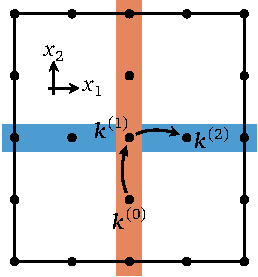
\includegraphics{chainDefinition_1}%
  }%
  \hfill%
  \subcaptionbox{%
    $d = 2$, $(t_1, t_2) = (1, 2)$%
    \label{fig:chainDefinition2}%
  }[47mm]{%
    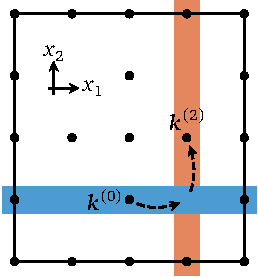
\includegraphics{chainDefinition_2}%
  }%
  \hfill%
  \subcaptionbox{%
    $d = 3$, $(t_1, t_2, t_3) = (2, 3, 1)$%
  }[50mm]{%
    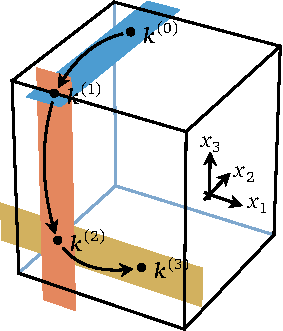
\includegraphics{chainDefinition_3}%
  }%
  \caption[%
    Examples for the definition of chains%
  ]{%
    Examples for chains in two and three dimensions.
    \emph{Left:} A chain from $\chain{0}$ to $\chain{2}$
    with respect to $(t_1, t_2) = (2, 1)$ in a two-dimensional sparse grid.
    \emph{Center:}
    With respect to the reverse permutation
    $(t_1, t_2) = (1, 2)$ of the dimensions,
    there is no chain from $\chain{0}$ to $\chain{2}$,
    because the corresponding chain point $\chain{1}$ is missing in the grid.
    \emph{Right:} A chain in three dimensions.%
  }%
  \label{fig:chainDefinition}%
\end{figure}

We now show two lemmas.
First, we prove that $(\upop{t_1,\dotsc,t_j})_{\*k'',\*k'} \not= 0$
is sufficient for the existence of a chain from $\*k'$ to $\*k''$:

\begin{restatable}[sufficient condition for chain existence]{%
  lemma%
}{%
  lemmaChainExistenceSufficient%
}
  \label{lemma:chainExistenceSufficient}
  If $(\upop{t_1,\dotsc,t_j})_{\*k'',\*k'} \not= 0$
  for some $j = 0, \dotsc, d$,
  then the grid $\liset$ contains the chain from $\*k'$ to $\*k''$
  with respect to $(t_1, \dotsc, t_j)$.
\end{restatable}

\vspace{-0.5em}

\begin{proof}
  See \cref{sec:a134proofCorrectnessUnidirectionalPrincipleSASG}.
\end{proof}

\vspace{0.5em}

Second, we show that the equality of
$(\upop{t_1,\dotsc,t_j})_{\chain{j},\*k'}$ and the product of
the one-dimensional operators is necessary for the
existence of a chain from $\*k'$ to $\*k''$:

\begin{restatable}[necessary condition for chain existence]{%
  lemma%
}{%
  lemmaChainExistenceNecessary%
}
  \label{lemma:chainExistenceNecessary}
  If the grid $\liset$ contains the chain $(\chain{0}, \dotsc, \chain{j})$
  from $\*k'$ to $\*k''$ with respect to $(t_1, \dotsc, t_j)$
  for some $j = 0, \dotsc, d$, then
  \begin{equation}
    \label{eq:lemmaChainExistenceNecessary}
    (\upop{t_1,\dotsc,t_j})_{\chain{j},\*k'}
    = (\upopuv{t_1}{\eqclass{\chain{1}}{\samepole{t_1}}})_{k''_{t_1},k'_{t_1}}
    \dotsm
    (\upopuv{t_j}{\eqclass{\chain{j}}{\samepole{t_j}}})_{k''_{t_j},k'_{t_j}}.
  \end{equation}
\end{restatable}

\vspace{-0.5em}

\begin{proof}
  See \cref{sec:a134proofCorrectnessUnidirectionalPrincipleSASG}.
\end{proof}

\vspace{0.5em}

These two lemmas can be used to prove the following characterization
of the correctness of the \up\punctfix{.}
Here, we need an additional assumption on the structure of the
operator $\linop$, which we call \term{tensor product structure:}

\begin{restatable}[characterization of the correctness of the UP]{%
  proposition%
}{%
  propCorrectnessUPCharacterization%
}
  \label{prop:correctnessUPCharacterization}
  Let $\linop$ have tensor product structure:
  For all $\*k', \*k'' \in \liset$ with the chain
  $(\chain{0}, \dotsc, \chain{d})$ from $\*k'$ to $\*k''$
  with respect to $(t_1, \dotsc, t_d)$,
  we assume that
  \begin{equation}
    \label{eq:tensorProductOperator}
    (\linop)_{\*k'',\*k'}
    = \prod_{j=1}^d
    (\upopuv{t_j}{\eqclass{\chain{j}}{\samepole{t_j}}})_{k''_{t_j},k'_{t_j}}.
  \end{equation}
  Then the \up is correct for $\linop$ and $(t_1, \dotsc, t_d)$
  if and only if the grid $\liset$ contains the chain from $\*k'$ to $\*k''$
  with respect to $(t_1, \dotsc, t_d)$ for all $\*k', \*k'' \in \liset$
  for which $(\linop)_{\*k'',\*k'} \not= 0$.
\end{restatable}

\vspace{-0.5em}

\begin{proof}
  See \cref{sec:a134proofCorrectnessUnidirectionalPrincipleSASG}.
\end{proof}

\vspace{0.5em}

When applied to the hierarchization operator,
the combination of \cref{prop:correctnessUPCharacterization} with
\thmref{lemma:dualityUnidirectionalPrinciple} can be summarized in
the following corollary:

\begin{corollary}[%
  equivalent statements for correctness of UP for hierarchization%
]
  \label{cor:equivalentCorrectnessUPHierarchization}
  The following statements are equivalent:
  \begin{itemize}
    \item
    The \up is correct for $\intpmatinv$ and $(t_1, \dotsc, t_d)$.
    
    \item
    The \up is correct for $\intpmat$ and $(t_d, \dotsc, t_1)$.
    
    \item
    The grid $\liset$ contains the chain from $\*k'$ to $\*k''$
    with respect to $(t_d, \dotsc, t_1)$ for all $\*k', \*k'' \in \liset$
    for which $\basis{\*k'}(\gp{\*k''}) \not= 0$.
  \end{itemize}
\end{corollary}

\begin{proof}
  The corollary is a direct consequence of
  \cref{lemma:dualityUnidirectionalPrinciple} and
  \cref{prop:correctnessUPCharacterization},
  applied to the dehierarchization operator $\linop = \intpmat$.
  
  The assumption of \cref{lemma:dualityUnidirectionalPrinciple}
  is satisfied:
  The operators $\upopuv{t_j}{\lisetpole}$ are invertible
  for all poles $\lisetpole$ in $\liset$
  due to the uniqueness of univariate interpolants
  (linear independence of the basis functions).
  Similarly, $\linop$ is invertible
  due to the uniqueness of multivariate interpolants.
  In addition, the assumption of \cref{prop:correctnessUPCharacterization}
  is satisfied, since
  \begin{equation}
    (\linop)_{\*k'',\*k'}
    = (\intpmat)_{\*k'',\*k'}
    = \prod_{j=1}^d \basis{k'_{t_j}}(\gp{k''_{t_j}})
    = \prod_{j=1}^d
    (\upopuv{t_j}{\eqclass{\chain{j}}{\samepole{t_j}}})_{k''_{t_j},k'_{t_j}}
  \end{equation}
  due to the tensor product basis functions.
\end{proof}

\paragraph{Inserting chain points}

This means that we can establish the correctness of the \up
for the hierarchization operator $\linop = \intpmatinv$,
if we insert all missing chain points that are specified by
\cref{prop:correctnessUPCharacterization} into the grid.

We take the case $p = 1$ of piecewise linear
standard B-splines $\bspl{\*l,\*i}{1}$ as an example.
We assume that we iteratively generated a spatially adaptive sparse grid
such that all grid points are reachable from the corners of $\clint{\*0, \*1}$
in the sense of \cref{eq:bfsAssumption2}.
If we want to ensure the correctness of the \up for all possible permutations
$(t_1, \dotsc, t_d)$ of the dimensions $(1, \dotsc, d)$,
then the existence of the necessary chains in
\cref{cor:equivalentCorrectnessUPHierarchization} is equivalent to the
requirement that the grid should contain
the hierarchical ancestors of every grid point in every direction:
\begin{subequations}
  \begin{alignat}{4}
    \fafa{(\*l',\*i') \in \liset}{\{t = 1, \dotsc, d \mid l'_t > 1\}}{
      (\*l,\*i) \in \liset
    },\quad
    &&&\*l \ceq \*l' - \stdbasis{t},\quad
    &&i_t \ceq 2 \floor{\tfrac{i'_t}{4}} + 1,\quad
    &&\*i_{-t} = \*i'_{-t},\\
    \fafa{(\*l',\*i') \in \liset}{\{t = 1, \dotsc, d \mid l'_t = 1\}}{
      (\*l,\*i) \in \liset
    },\quad
    &&&\*l \ceq \*l' - \stdbasis{t},\quad
    &&i_t \ceq 0,\quad
    &&\*i_{-t} = \*i'_{-t},
  \end{alignat}
\end{subequations}
where $\stdbasis{t}$ is the $t$-th standard basis vector.
This is a standard assumption on spatially adaptive sparse grids with
piecewise linear basis functions \cite{Pflueger10Spatially}.
However, we only have to satisfy the conditions of
\cref{cor:equivalentCorrectnessUPHierarchization} for a single permutation
$(t_1, \dotsc, t_d)$ of the dimensions
in order to hierarchize with the \up\punctfix{.}
\Cref{fig:chainInsertionBSpline} shows the necessary ancestor chain points
(colored points in \cref{fig:chainInsertionBSpline2})
for an example of a two-dimensional spatially adaptive sparse grid
(\cref{fig:chainInsertionBSpline1}).

\begin{figure}
  \subcaptionbox{%
    Original grid ($N = 85$)%
    \label{fig:chainInsertionBSpline1}%
  }[48mm]{%
    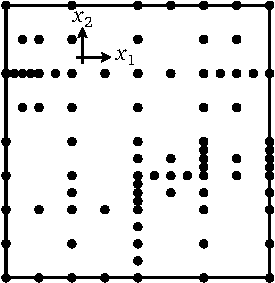
\includegraphics{chainInsertion_1}%
  }%
  \hfill%
  \subcaptionbox{%
    Chain points for $p = 1$\\
    \rlap{\hspace*{10.5mm}($N = 121$)}%
    \label{fig:chainInsertionBSpline2}%
  }[48mm]{%
    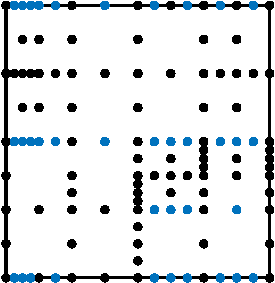
\includegraphics{chainInsertion_2}%
  }%
  \hfill%
  \subcaptionbox{%
    Chain points for $p = 3$\\
    \rlap{\hspace*{10.5mm}($N = 289 = 17 \times 17$)}%
    \label{fig:chainInsertionBSpline3}%
  }[48mm]{%
    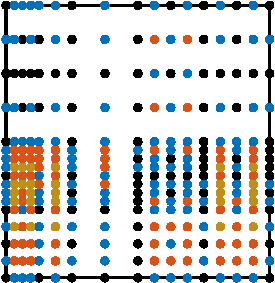
\includegraphics{chainInsertion_3}%
  }%
  \caption[%
    Chain points for hierarchical B-splines on a sparse grid%
  ]{%
    Necessary chain points for the correctness of the unidirectional principle
    with respect to $(t_1, t_2) = (1, 2)$
    for hierarchical B-splines $\bspl{l,i}{p}$ on a
    two-dimensional spatially adaptive sparse grid.
    The colors indicate the recursion depth in which the
    chain points have been inserted.
    Black points are contained in the original grid
    (``zero-order points'').
    \textcolor{C0}{Blue points} are part of chains
    between original grid points (``first-order chain points'').
    \textcolor{C1}{Red points} are second-order chain points,
    i.e., they are part of chains
    from $\*k'$ to $\*k''$ where $\*k'$ and $\*k''$ are
    original grid points or first-order chain points
    and at least one of them is a first-order chain point.
    Analogously,
    \textcolor{C2}{brown points} are third-order chain points.
    $N$ is the number of points in the final grid.%
  }%
  \label{fig:chainInsertionBSpline}%
\end{figure}

Unfortunately, we have to insert these points recursively,
e.g., the inserted points may generate new chains,
for which other missing points have to be inserted and so on
(``higher-order chain points'' in \cref{fig:chainInsertionBSpline}).
Therefore, the number of points to be inserted may be large.
The worst case is that the final grid is a full grid, i.e.,
the Cartesian product of the union of the poles in the different dimensions:
\begin{equation}
  \paren*{\bigcup_{\*k \in \liset} \eqclass{\*k}{\samepole{1}}}
  \times \dotsb \times
  \paren*{\bigcup_{\*k \in \liset} \eqclass{\*k}{\samepole{d}}},
\end{equation}
i.e., we fully lose the advantage of sparse grids,
whose purpose is to ease the curse of dimensionality.
For the standard hierarchical B-spline basis $\bspl{l,i}{p}$,
this worst case often occurs as there are many non-zero entries
in the corresponding interpolation matrices $\intpmat$
(see \cref{sec:41problem} and \cref{fig:chainInsertionBSpline3}).



\subsection{Hierarchical Weakly Fundamental Splines}
\label{sec:454wfs}

\paragraph{Motivation}

In order to reduce the number of chain points to be inserted,
we have to use other spline bases such that
the resulting interpolation matrices $\intpmat$ have more zero entries.
The hierarchical fundamental splines
as introduced in \cref{sec:443fundamentalSplines} are one possibility.
However, they are globally supported, which implies a number
of disadvantages concerning the algorithms and the implementations.
The most significant disadvantage is that although
we can use \bfs for the univariate hierarchization operators,
the time complexity for the univariate hierarchization is still quadratic.
We search for a locally supported spline basis for which
the univariate hierarchization can be done in linear time.

To meet these goals, we have to relax the fundamental property
to a weaker version, which results in the so-called
\term{weakly fundamental property.}
A univariate hierarchical basis
$\wfundbasis{l',i'}\colon \clint{0, 1} \to \real$
is called \term{weakly fundamental,} if
\begin{equation}
  \label{eq:weaklyFundamentalProperty}
  \wfundbasis{l',i'}(\gp{l,i}) = 0,\quad
  l < l',\;\;
  i \in \hiset{l}.
\end{equation}
This is exactly the first condition \eqref{eq:fundamentalProperty1}
of the fundamental property \eqref{eq:fundamentalProperty}.
We drop the requirement that the basis functions
should vanish at the other grid points of the same level.
The relation \eqref{eq:fundamentalPropertyImplicationMV} from the
fundamental case becomes
\begin{equation}
  \label{eq:weaklyFundamentalPropertyImplicationMV}
  \wfundbasis{\*l',\*i'}(\gp{\*l,\*i})
  \not= 0
  \implies
  \*l' \le \*l,
\end{equation}
i.e., every basis function $\wfundbasis{\*l',\*i'}$
can only be non-zero at grid points $\gp{\*l,\*i}$ with
higher or equal level $\*l$.

\paragraph{Definition of hierarchical weakly fundamental splines}

We construct the \term{weakly fundamental spline parent function}
$\parentwfundspl{p}\colon \real \to \real$
by forming a linear combination of as few neighboring
uniform B-splines as possible such that $\parentwfundspl{p}$
satisfies the weakly fundamental property
\eqref{eq:weaklyFundamentalProperty}:
\begin{subequations}
  \begin{gather}
    \label{eq:weaklyFundamentalSplineParent}
    \parentwfundspl{p}(x)
    \ceq \largesum[(p-1)/2]{k=-(p-1)/2}
    \wfundsplcoeff{k}{p} \parentbspl{p}(x - k)
    \quad\text{such that}\\
    \wfundsplcoeff{0}{p} = 1,\quad
    \parentwfundspl{p}(k') = 0,\;\;
    k' = -p + 2,\; -p + 4,\; \dotsc,\; p - 2.
  \end{gather}
\end{subequations}
\usenotation{zzzzwfs}
\term{Hierarchical weakly fundamental splines}
$\bspl[\wfs]{l,i}{p}\colon \clint{0, 1} \to \real$
are now defined canonically via an affine parameter transformation:
\begin{equation}
  \bspl[\wfs]{l,i}{p}(x)
  \ceq \parentwfundspl{p}(\tfrac{x}{\ms{l}} - i),\quad
  l \ge 1.
\end{equation}
For $l = 0$, we define $\bspl[\wfs]{l,i}{p}$ to be the
linear Lagrange polynomial of level zero:%
\footnote{%
  This will simplify the description of the
  Hermite hierarchization algorithm in \cref{sec:455hermiteHierarchization}.%
}
\begin{equation}
  \bspl[\wfs]{0,i}{p}
  \ceq \lagrangepoly{0,i},\quad
  i = 0, 1.
\end{equation}
The hierarchical weakly fundamental spline basis is shown in
\cref{fig:hierarchicalWeaklyFundamentalSpline}.
Note that these basis functions are translation-invariant by construction
(starting with level $l \ge 1$).
As the weakly fundamental parent spline $\parentwfundspl{p}$
vanishes at all odd integers and as the
support of $\bspl[\wfs]{l,i}{p}$ is local
($\supp \bspl[\wfs]{l,i}{p}
= \clint{\gp{l,i-p}, \gp{l,i+p}} \cap \clint{0, 1}$),
this implies that the weakly fundamental property
\eqref{eq:weaklyFundamentalProperty} is fulfilled.

\begin{SCfigure}
  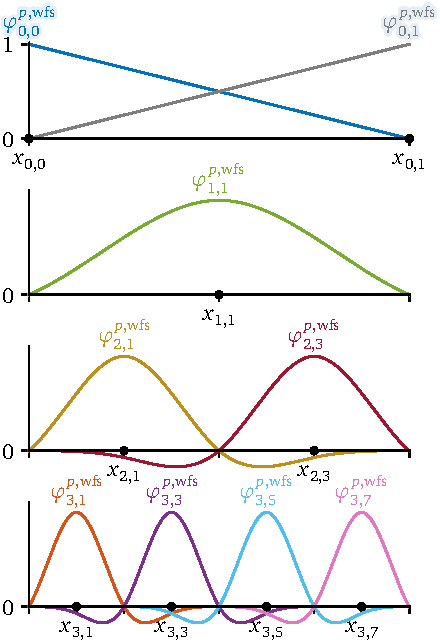
\includegraphics{hierarchicalBasis_17}%
  \caption[%
    Hierarchical weakly fundamental splines%
  ]{%
    Hierarchical cubic weakly
    \vspace{-0.1em}%
    fundamental splines
    $\bspl[\wfs]{l',i'}{p}$
    ($l' \le l$, $i' \in \hiset{l'}$, $p = 3$) and
    grid points $\gp{l',i'}$ \emph{(dots)} up to level $l = 3$.%
  }%
  \label{fig:hierarchicalWeaklyFundamentalSpline}%
\end{SCfigure}

\paragraph{Chain points for weakly fundamental splines}

The first advantage of the
weakly fundamental spline basis $\bspl[\wfs]{l,i}{p}$
over standard uniform B-splines $\bspl{l,i}{p}$ is that
the condition $\basis{\*k'}(\gp{\*k''}) \not= 0$ in
\cref{cor:equivalentCorrectnessUPHierarchization} is
satisfied for much fewer $\*k', \*k''$.
Consequently, fewer chain grid points have to be inserted to
ensure the correctness of the \up for hierarchization.
\Cref{fig:chainInsertionWeaklyFundamentalSpline} shows the inserted points
for the same grid as in \cref{fig:chainInsertionBSpline}.

\begin{SCfigure}
  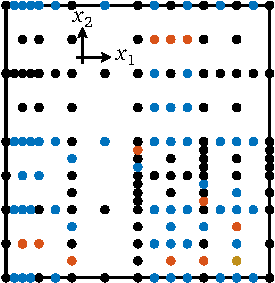
\includegraphics{chainInsertion_4}%
  \caption[%
    Chain points for hierarchical weakly fundamental splines on a
    sparse grid%
  ]{%
    Necessary chain points for the correctness of the unidirectional principle
    with respect to $(t_1, t_2) = (1, 2)$
    for hierarchical cubic weakly fundamental splines
    $\bspl[\wfs]{l,i}{p}$ ($p = 3$)
    on the same two-dimensional spatially adaptive sparse grid
    as in \cref{fig:chainInsertionBSpline1}.
    The colors indicate the recursion depth in which the
    chain points have been inserted
    (see caption of \cref{fig:chainInsertionBSpline}).
    The number of points in the final grid is $N = 157$.%
  }%
  \label{fig:chainInsertionWeaklyFundamentalSpline}%
\end{SCfigure}

In the special case of regular sparse grids $\regsgset{n}{d}$,
we do not have to insert any grid points for the correctness of the
\up\punctfix{.}
We can verify this statement with
\thmref{cor:equivalentCorrectnessUPHierarchization}:
Let $(\*l',\*i')$ and $(\*l'',\*i'')$ with
$\normone{\*l'}, \normone{\*l''} \le n$ and
$\*i' \in \hiset{\*l'}$, $\*i'' \in \hiset{\*l''}$,
such that $\bspl[\wfs]{\*l',\*i'}{p}(\gp{\*l'',\*i''}) \not= 0$.
Furthermore, let $(\chain[\*l]{0}, \chain[\*i]{0}), \dotsc,
(\chain[\*l]{d}, \chain[\*i]{d})$ be the chain
from $\*k'$ to $\*k''$ with respect to $t_1, \dotsc, t_d$.
Note that $\chain[\*l]{j} \le \vecmax\{\*l', \*l''\}$ due to the
definition of chain points (\cref{def:chain}).
Therefore, we have for $j = 0, \dotsc, d$
by \eqref{eq:weaklyFundamentalPropertyImplicationMV}:
\begin{equation}
\*l' \le \*l''
\implies
\chain[\*l]{j} \le \vecmax\{\*l', \*l''\} \le \*l''
\implies
\normone{\chain[\*l]{j}} \le \normone{\*l''} \le n.
\end{equation}
Hence, $\regsgset{n}{d}$ contains the grid points corresponding to
$(\chain[\*l]{j}, \chain[\*i]{j})$ for all $j = 0, \dotsc, d$.
Consequently, the conditions of
\cref{cor:equivalentCorrectnessUPHierarchization} are satisfied without
inserting any additional chain points.
This statement is even valid for arbitrary
dimensionally adaptive sparse grids.



\subsection{Hermite Hierarchization}
\label{sec:455hermiteHierarchization}

\paragraph{Hermite interpolation}

The second advantage of the weakly fundamental spline basis
is that due to the reduced coupling,
the univariate hierarchization operators can be applied easier
than for standard uniform B-splines.
This results in the formulation of the so-called
\term{Hermite hierarchization} algorithm.
We first recall higher-order Hermite interpolation:

\begin{lemma}[higher-order Hermite interpolation]
  \label{lemma:hermiteInterpolation}
  Let $p \in \nat$ be odd and $a, b \in \real$ with $a < b$.
  Furthermore, let
  $\deriv[q]{x}{\objfun}(a) \in \real$ and
  $\deriv[q]{x}{\objfun}(b) \in \real$ be given data
  for $q = 0, \dotsc, \frac{p-1}{2}$.
  Then there is a unique polynomial $\spl \in \polyspace{p}$ such that
  \begin{equation}
    \deriv[q]{x}{\objfun}(a)
    = \deriv[q]{x}{\spl}(a),\quad
    \deriv[q]{x}{\objfun}(b)
    = \deriv[q]{x}{\spl}(b),\quad
    q = 0, \dotsc, \frac{p-1}{2}.
    \hspace*{-10mm}
  \end{equation}
\end{lemma}

\begin{proof}
  See \cite{Freund07Stoer}.
\end{proof}

\paragraph{Hermite hierarchization algorithm}

The interpolating polynomial $\spl$ and its derivatives can be
efficiently evaluated using Hermite basis functions
(generalized Lagrange polynomials \cite{Freund07Stoer}).
With Hermite interpolation, we formulate
\cref{alg:hermiteHierarchization}
for the hierarchization with hierarchical weakly fundamental splines.
While we formulate \cref{alg:hermiteHierarchization}
only for regular univariate grids and weakly fundamental splines,
a slightly reformulated version of the algorithm
also correctly operates on spatially adaptive univariate grids
(with the assumption that the grids contain the parents of their grid points)
and other weakly fundamental bases that are
piecewise polynomials of degree $\le p$.

\begin{algorithm}
  \begin{algorithmic}[1]
    \Function{$\vlinout = \texttt{hermiteHierarchization1D}$}{%
      $\vlinin$, $n$%
    }
      \For{$i = 0, 1$}
      \Comment{set values for level $0$}%
        \State{%
          $\linout{0,i} \gets \fcnval{0,i}$%
        }
        \label{line:algHermiteHierarchization1}
        \State{%
          $\deriv[q]{x}{\fgintp{0}}(\gp{0,i})
          \gets \kronecker{q}{0} \cdot \fcnval{0,i} +
          \kronecker{q}{1} \cdot (\fcnval{0,1} - \fcnval{0,0})$
          for all $q = 0, \dotsc, \frac{p-1}{2}$%
        }
        \label{line:algHermiteHierarchization3}
      \EndFor{}
      \For{$l = 1, \dotsc, n$}
        \For{$i \in \hiset{l}$}
          \State{%
            $\fgintp{l-1}(\gp{l,i}) \gets \text{Hermite interpolation of}$
            $\deriv[q]{x}{\fgintp{l-1}}(\gp{l,i\pm1})$
            ($q = 0, \dotsc, \frac{p-1}{2}$)%
          }
          \label{line:algHermiteHierarchization4}
          \State{%
            $r^{(l)}(\gp{l,i})
            \gets \fcnval{l,i} - \fgintp{l-1}(\gp{l,i})$%
          }
          \label{line:algHermiteHierarchization5}
          \Comment{residual to be interpolated}%
        \EndFor{}
        \State{%
          Let $r^{(l)}_l$ be of the form
          $\sum_{i' \in \hiset{l}} \linout{l,i'} \bspl[\wfs]{l,i'}{p}$%
        }
        \Comment{contribution of level $l$}%
        \label{line:algHermiteHierarchization6}
        \State{%
          Choose $(\linout{l,i'})_{i' \in \hiset{l}}$ such that
          $r^{(l)}_l(\gp{l,i}) = r^{(l)}(\gp{l,i})$ for all $i \in \hiset{l}$%
        }
        \label{line:algHermiteHierarchization7}
        \For{$i = 0, \dotsc, 2^l$}
        \Comment{for all points (current level and ancestors)}%
          \For{$q = 0, \dotsc, \frac{p-1}{2}$}
            \State{%
              $\deriv[q]{x}{\fgintp{l}}(\gp{l,i})
              \gets \deriv[q]{x}{\fgintp{l-1}}(\gp{l,i}) +
              \deriv[q]{x}{r^{(l)}_l}(\gp{l,i})$%
            }
            \Comment{update values}%
            \label{line:algHermiteHierarchization8}
          \EndFor{}
        \EndFor{}
      \EndFor{}
    \EndFunction{}
  \end{algorithmic}
  \caption[%
    Hermite hierarchization%
  ]{%
    Hermite hierarchization on one-dimensional regular grids.
    Inputs are
    the vector $\vlinin = (\linin{l,i})_{(l,i) \in \liset}$
    of input data (function values $\fcnval{l,i}$ at the grid points) and
    the level $n$ of the regular grid,
    where $\liset = \{(l, i) \mid l = 0, \dotsc, n,\; i \in \hiset{l}\}$.
    The output is the vector
    $\vlinout = (\linout{l,i})_{(l,i) \in \liset}$
    of output data (hierarchical surpluses $\surplus{l,i}$).%
  }%
  \label{alg:hermiteHierarchization}%
\end{algorithm}

\vspace*{\fill}

The idea of \cref{alg:hermiteHierarchization},
which is also illustrated in \cref{fig:hermiteHierarchization},
is to hierarchize the function value data level by level,
which is only possible because of the weakly fundamental property
\eqref{eq:weaklyFundamentalProperty}.
For each level $l$, we calculate surpluses
$\surplus{l,i} = \linout{l,i}$, while keeping track of
the values and derivatives
$\deriv[q]{x}{\fgintp{l}}(\gp{l,i})$ of the
``current'' interpolant $\fgintp{l}$ (up to level $l$).
Hermite interpolation is used to determine the ``delta''
to the interpolant of the next level.
Note that in \cref{line:algHermiteHierarchization8},
we have to evaluate the derivatives of
$\deriv[q]{x}{\fgintp{l-1}}(\gp{l,i})$ of the Hermite interpolant
determined in \cref{line:algHermiteHierarchization4}.
This is not an issue since in an implementation
one would typically simultaneously evaluate the
Hermite interpolant and its derivatives.

\vspace*{\fill}

\begin{SCfigure}
  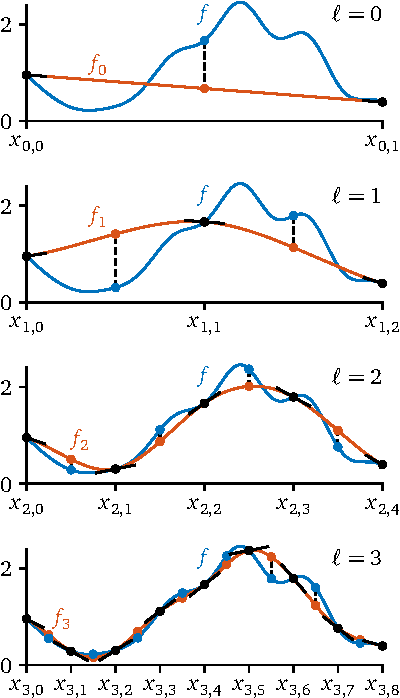
\includegraphics{hermiteHierarchization_1}%
  \caption[%
    Hermite hierarchization%
  ]{%
    Hermite hierarchization on a regular grid in one dimension
    with cubic weakly fundamental splines $\bspl[\wfs]{l,i}{p}$ ($p = 3$).
    The interpolants $\fgintp{l}$ \emph{\textcolor{C1}{(red)}}
    of the objective function \emph{\textcolor{C0}{(blue)}}
    are computed level by level.
    For each level $l$,
    \vspace{-0.1em}%
    the values $\fgintp{l}(\gp{l,i})$ and the derivatives
    $\deriv{x}{\fgintp{l}}(\gp{l,i})$ of the
    current interpolant $\fgintp{l}$ at the
    grid points $\gp{l,i}$ ($i = 0, \dotsc, 2^l$) are saved
    \emph{(black dots and bars).}
    The values and derivatives are used for the Hermite interpolation
    of the residual $\objfun - \fgintp{l}$.
    The interpolated residual is then added to the current interpolant
    such that the sum vanishes in the grid points of the next level $l + 1$
    \emph{%
      (black dashed lines between \textcolor{C1}{red} and
      \textcolor{C0}{blue} dots).%
    }
    Due to the weakly fundamental property, the previously
    interpolated values of $\objfun$ remain unchanged.%
  }%
  \label{fig:hermiteHierarchization}%
\end{SCfigure}

For hierarchical weakly fundamental splines,
the complexity of the $l$-th iteration of \cref{alg:hermiteHierarchization}
is linear in the number of grid points of level $l$, i.e., $\landauO{2^l}$.
The reason for this is the bandedness (with bandwidth $\landauO{p}$) of the
system of linear equations corresponding to the interpolation problem of
\cref{line:algHermiteHierarchization6,line:algHermiteHierarchization7},
which means that the interpolation problem can be solved in
linear time and memory.
In total, the complexity of \cref{alg:hermiteHierarchization} is
given by $\landauO{\sum_{l=0}^n 2^l} = \landauO{2^n}$, i.e.,
the time and memory required by \cref{alg:hermiteHierarchization}
is only linear in the number of grid points.

\pagebreak

\paragraph{Correctness}

We prove the correctness of Hermite hierarchization
with the following invariant.

\begin{restatable}[invariant of Hermite hierarchization]{%
  proposition%
}{%
  propInvariantHermiteHierarchization%
}
  \label{prop:invariantHermiteHierarchization}
  In \cref{alg:hermiteHierarchization}, it holds
  for $l = 0, \dotsc, n$ and $i = 0, \dotsc, 2^l$
  \begin{equation}
    \label{eq:propInvariantHermiteHierarchization}
    \deriv[q]{x}{\fgintp{l}}(\gp{l,i})
    = \sum_{l'=0}^l \sum_{i' \in \hiset{l'}}
    \linout{l',i'} \deriv[q]{x}{\bspl[\wfs]{l',i'}{p}}(\gp{l,i}),\quad
    q = 0, \dotsc, \frac{p-1}{2}.
    \hspace*{-6mm}
  \end{equation}
\end{restatable}

\begin{proof}
  See \cref{sec:a135proofHermiteHierarchization}.
\end{proof}

\begin{restatable}[correctness of Hermite hierarchization]{%
  shortcorollary%
}{%
  corAlgHermiteHierarchizationCorrectness%
}
  \label{cor:algHermiteHierarchizationCorrectness}
  \Cref{alg:hermiteHierarchization} is correct.
\end{restatable}

\begin{proof}
  See \cref{sec:a135proofHermiteHierarchization}.
\end{proof}



\subsection{Hierarchical Weakly Fundamental Not-A-Knot Splines}
\label{sec:456wfsNotAKnot}

Finally, as for fundamental splines,
it is possible to combine the weakly fundamental basis
with the not-a-knot idea from \cref{sec:32notAKnot} to construct
hierarchical weakly fundamental not-a-knot spline functions
$\bspl[\wfs,\nak]{l',i'}{p}$.
The approach is similar to the fundamental not-a-knot splines
in \cref{sec:445fundamentalNotAKnotSplines}
(see \cref{eq:fundamentalNotAKnotSplines}):
Instead of combining uniform B-splines as in
\eqref{eq:weaklyFundamentalSplineParent},
we combine not-a-knot B-splines such that the
weakly fundamental property is satisfied.

However, the exact construction is somewhat complicated,
as one has to carefully consider which conditions to enforce
with which basis functions.
There are some special cases, if the index of the basis function
$\bspl[\wfs,\nak]{l',i'}{p}$ is near the boundary
(near $i' = 0$ or near $i' = 2^{l'}$).
Nevertheless, there are only finitely many special cases;
for higher levels $l'$, one can just scale the basis functions
of coarser levels.
In the scope of this thesis,
it suffices to show the resulting basis functions for
the cubic case ($p = 3$) in
\cref{fig:hierarchicalWeaklyFundamentalNotAKnotSpline},
instead of rigorously stating the technical formulas.

\begin{SCfigure}
  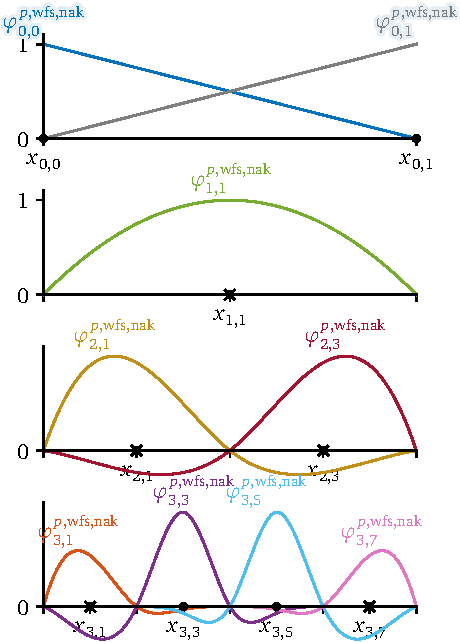
\includegraphics{hierarchicalBasis_18}%
  \caption[%
    Hierarchical weakly fundamental not-a-knot splines%
  ]{%
    Hierarchical cubic weakly fundamental not-a-knot splines
    $\bspl[\wfs,\nak]{l',i'}{p}$
    ($l' \le l$, $i' \in \hiset{l'}$, $p = 3$),
    grid points $\gp{l',i'}$ \emph{(dots),} and
    removed knots \emph{(crosses)} up to level $l = 3$.%
  }%
  \label{fig:hierarchicalWeaklyFundamentalNotAKnotSpline}%
\end{SCfigure}
